\chapter{Hauptkomponentenanalyse}   

Die Hauptkomponentenanalyse (engl.\ \emph{Principal Component Analysis}, PCA) ist ein Verfahren zur Dimensionsreduktion von Daten.
Genauer: Es handelt sich um eine Methode, um komplexe Daten auf ihr Wesentliches zu reduzieren, was eine Weiterverarbeitung und Visualisierung erleichtert.

In diesem Kapitel wird zunächst die Intuition hinter der PCA erläutert, bevor der mathematische Hintergrund und insbesondere die Verbindung zur Singulärwertzerlegung beschrieben wird.
Abschließend betrachten wir ein konkretes Anwendungsbeispiel und veranschaulichen dieses mithilfe der Programmiersprache \texttt{Python}.

\section{Intuition der PCA}\label{sec:pcaint}
Angenommen, beim Familienessen käme die Frage auf, welche der mitgebrachten Weine sich am ähnlichsten sind. 
Um diese Frage zu beantworten, überlegt sich die Familie verschiedene Merkmale und ordnet jedem Wein für jedes Merkmal Zahlen zwischen \num{-3} und \num{3} zu.
Dadurch können die Weine als Punkte im Raum bezüglich der verschiedenen Werte dargestellt und anschließend analysiert werden, welche Weine sich gruppieren, also sich ähneln. 

In \zcref{fig:pcadim}, zu finden im \zcref{appen}, wird dies für verschiedene \(n \coloneqq \emph{Anzahl der Merkmale}\) verdeutlicht. 

Das Problem wird schnell ersichtlich:
Eine visuelle Interpretation ist zwar möglich, allerdings nur im niedrig-dimensionalen Raum, für eine größere Anzahl an Merkmalen (Dimensionen) besteht die Notwendigkeit, die Anzahl zu reduzieren.
Diese Dimensionsreduktion stellt in vielen Fällen auch unabhängig von der visuellen Interpretation eine sinnvolle Maßnahme dar.
In Bezug auf unser Beispiel bestehe die Möglichkeit, dass \enquote{Alkoholgehalt} und \enquote{Schwere} stark korrelieren und somit redundant für eine Rekonstruktion der Weine sind.
Eine andere Möglichkeit zur Reduzierung der Merkmale ist dadurch gegeben, dass gewisse Merkmale wenig Informationen über die Charakteristiken der Weine enthalten, wie beispielsweise die Flaschenform oder die Fließgeschwindigkeit.

Die Hauptkomponentenanalyse konstruiert neue, unkorrelierte Richtungen, die sich als Linearkombinationen aus den bestehenden Merkmalen zusammensetzen.
Dadurch könnten beispielsweise \enquote{Alkoholgehalt} und \enquote{Schwere} zu einer neuen \emph{Hauptrichtung} zusammengefasst werden.
Anschließend werden die Weine auf den durch diese Richtung definierten Unterraum projiziert.
Die projizierten Koordinaten entlang dieser neuen Achse ergeben die erste \emph{Hauptkomponente} (PC1).
Der Unterschied zwischen Hauptrichtung und Hauptkomponente wird am Ende der Intuition präzisiert.

Die Projektion wird in \zcref{fig:pca2d} veranschaulicht.
\begin{figure}[bt]
    \centering
    \begin{subfigure}{\textwidth}
        \centering
        \caption{}\label{fig:pca2d1}
        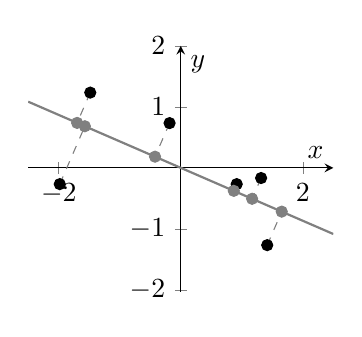
\begin{tikzpicture}[baseline]
        \begin{axis}[
            xlabel={\(x\)},
            ylabel={\(y\)},
            axis y line=center,
            axis x line=middle,
            axis equal,
            width=0.45\textwidth,
            xmin=-2.5,
            xmax=2.5
        ]
        \addplot[only marks,mark options={fill=black, color=black},domain=-2:2] coordinates {
            (1.4167,-1.2667)
            (-1.4833,1.2333)
            (1.3167,-0.1667)
            (-1.9833,-0.2667)
            (0.9167,-0.2667)
            (-0.1833,0.7333)                
        };
        \addplot[Gray, thick, domain=-2.5:2.5] {-0.4337*x};

        \addplot[only marks, mark options={fill=Gray, color=Gray}] coordinates {
            ( 1.65481157, -0.71762599)
            (-1.69867778,  0.73664903)
            ( 1.16912424, -0.50700271)
            (-1.57200891,  0.68171777)
            ( 0.86894276, -0.37682593)
            (-0.42195053,  0.18298317)
        };
        \addplot[dashed, gray] coordinates {
            (1.4167, -1.2667) ( 1.65481157, -0.71762599)
        };
        \addplot[dashed, gray] coordinates {
            (-1.4833, 1.2333) (-1.69867778,  0.73664903)
        };
        \addplot[dashed, gray] coordinates {
            (1.3167, -0.1667) ( 1.16912424, -0.50700271)
        };
        \addplot[dashed, gray] coordinates {
            (-1.9833, -0.2667) (-1.57200891,  0.68171777)
        };
        \addplot[dashed, gray] coordinates {
            (0.9167, -0.2667) (0.86894276, -0.37682593)
        };
        \addplot[dashed, gray] coordinates {
            (-0.1833, 0.7333) (-0.42195053,  0.18298317)  
        };
        \end{axis}
    \end{tikzpicture}
        \hspace{20pt}
        \begin{tikzpicture}[baseline]
    \begin{axis}[
        xlabel={\(PC1\)},
        ylabel={},
        axis y line=center,
        axis x line=middle,
        axis equal,
        ytick=\empty,
        width=0.45\textwidth,
        xmin=-2.5,
        xmax=2.5
    ]
    \addplot[only marks, mark options={fill=black, color=black}] coordinates {
        ( 1.803, 0)
        (-1.849, 0)
        ( 1.279, 0)
        (-1.697, 0)
        ( 0.928, 0)
        (-0.469, 0)
    };


    \end{axis}
\end{tikzpicture}
    \end{subfigure}
    \begin{subfigure}{\textwidth}
        \centering
        \caption{}\label{fig:pca2d2}
        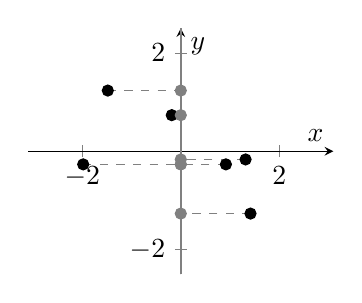
\begin{tikzpicture}[baseline]
    \begin{axis}[
        xlabel={\(x\)},
        ylabel={\(y\)},
        axis y line=center,
        axis x line=middle,
        axis equal,
        width=0.45\textwidth,
        xmin=-2.5,
        xmax=2.5
    ]
    \addplot[only marks,mark options={fill=black, color=black},domain=-2:2] coordinates {
        (1.4167,-1.2667)
        (-1.4833,1.2333)
        (1.3167,-0.1667)
        (-1.9833,-0.2667)
        (0.9167,-0.2667)
        (-0.1833,0.7333)                
    };
    \addplot[Gray, thick, domain=-2.5:2.5] ({0}, x);

    \addplot[only marks, mark options={fill=Gray, color=Gray}] coordinates {
        (0,-1.2667)
        (0,1.2333)
        (0,-0.1667)
        (0,-0.2667)
        (0,-0.2667)
        (0,0.7333)
    };
    \addplot[dashed, gray] coordinates {
        (1.4167, -1.2667) (0,-1.2667)
    };
    \addplot[dashed, gray] coordinates {
        (-1.4833, 1.2333) (0,1.2333)
    };
    \addplot[dashed, gray] coordinates {
        (1.3167, -0.1667) (0,-0.1667)
    };
    \addplot[dashed, gray] coordinates {
        (-1.9833, -0.2667) (0,-0.2667)
    };
    \addplot[dashed, gray] coordinates {
        (0.9167, -0.2667) (0,-0.2667)
    };
    \addplot[dashed, gray] coordinates {
        (-0.1833, 0.7333) (0,0.7333)  
    };
    \end{axis}
\end{tikzpicture}
        \hspace{20pt}
        \begin{tikzpicture}[baseline]
    \begin{axis}[
        xlabel={\(PC1\)},
        ylabel={},
        axis y line=center,
        axis x line=middle,
        axis equal,
        ytick=\empty,
        width=0.45\textwidth,
        xmin=-2.5,
        xmax=2.5
    ]
    \addplot[only marks, mark options={fill=black, color=black}] coordinates {
        (-1.2667,0)
        (1.2333,0)
        (-0.1667,0)
        (-0.2667,0)
        (-0.2667,0)
        (0.7333,0)
    };


    \end{axis}
\end{tikzpicture}
    \end{subfigure}
    \caption{Projektionen im zweidimensionalen Raum}\label{fig:pca2d}
\end{figure}
Der Unterschied zwischen \zcref{fig:pca2d1} und \zcref{fig:pca2d2} zeigt folgendes Problem auf:
Wie kann die neue Richtung optimal gewählt werden, sodass unsere Daten trotz der Dimensionsreduktion so originalgetreu wie möglich rekonstruiert werden können?
Dafür gibt es zwei alternative, aber äquivalente, Formulierungen:
\vspace{-2pt}
\begin{enumerate}
    \item Die Richtung wird so konstruiert, dass ein Minimum an Informationen verloren wird.
    \item Die Richtung wird so konstruiert, dass eine maximale Varianz erhalten bleibt.
\end{enumerate}
Eine Äquivalenz dieser beiden Aussagen kann durch den Satz des Pythagoras hergeleitet werden, indem das rechtwinklige Dreieck zwischen einem Punkt, dessen Projektion und dem Ursprung betrachtet wird. 
Wird der Informationsverlust (Distanz zwischen der Projektion und dem Original) minimiert, maximiert sich die Varianz (Abstand zum Ursprung).
Es sei angemerkt, dass dafür von einer Zentrierung der Daten ausgegangen wird, also von einem Mittelwert gleich null.

Mit diesem Hintergrund wird intuitiv ersichtlich, dass \zcref{fig:pca2d1} im Vergleich zu \zcref{fig:pca2d2} vorzuziehen ist, was sich im Ergebnis widerspiegelt, in dem die räumliche Verteilung im Wesentlichen erhalten bleibt.

In vielen mathematischen Texten erfolgt keine klare Differenzierung zwischen den Begriffen Hauptrichtung und Hauptkomponente.
Stattdessen wird der Begriff Hauptkomponente häufig synonym für beide verwendet.
In dieser Arbeit definieren wir die erste Hauptrichtung als den Einheitsvektor, der den eindimensionalen Unterraum aufspannt, auf den die Daten mit maximaler Varianz projiziert werden.
Die erste Hauptkomponente bezeichnet die projizierten Koordinaten der Datenpunkte entlang dieser Hauptrichtung.
In höheren Dimensionen wird die zweite Hauptrichtung so gewählt, dass sie orthogonal zur ersten Hauptrichtung liegt und die verbleibende Varianz maximiert.
Dies kann beliebig fortgesetzt werden, die PCA besitzt allerdings die nützliche Eigenschaft, dass die Hauptrichtungen nach \enquote{Wichtigkeit} sortiert sind, also die ersten Richtungen bereits den Großteil der Varianz erklären.
Eine genauere Erläuterung dieser Aussage wird dabei in der folgenden mathematischen Herleitung gegeben.

\section{Mathematische Herleitung}
Bevor die vorangegangenen Überlegungen formalisiert werden können, rekapitulieren wir durch \zcref{rep:proj} die Formel der orthogonalen Projektion.
\begin{repitition}\label{rep:proj}
    Sei \(n \in \N\) und \(u,x \in \R^{n}\) mit \(\norm{u} = 1\).  \\
    Dann ist der orthogonal projizierte Vektor \(\operatorname{proj}_{u}(x)\) von \(x\) auf \(u\) gegeben durch
    \begin{equation*}
        \operatorname{proj}_{u}(x) = \langle x,u \rangle u = (x^{T}u)u.
    \end{equation*}     
\end{repitition}
Das Ziel der Herleitung in diesem Abschnitt wird durch \zcref{app:pca} zusammengefasst.
\begin{application}[PCA]\label{app:pca}
    Seien \(n,d \in \N\) und  
    \begin{equation*}
        X = 
        \big[
            \begin{matrix}
                x_1 \dots x_d
            \end{matrix}    
        \big] \in \R^{n \times d}
    \end{equation*} 
    eine standardisierte\footnote{Siehe \hyperref[itm:pca1]{Schritt 1} im Beweis} Datenmatrix, die \(d\) Merkmale über \(n\) Objekte hinweg speichert und
    \begin{equation*}
        \R^{d} \ni x^{(i)} \coloneqq X_{i,:} \quad \text{für } i \in \{1,\ldots,n\},
    \end{equation*}
    die \(i\)-te (transponierte) Zeile von \(X\), also ein Datenpunkt.     \\
    Bei der Projektion der Daten auf \(\R^{k}\) für \(\N \ni k < d\) mit dem Ziel, dass die maximale Varianz der \(x^{(i)}\) erhalten bleiben soll, wird die Basis von \(\R^{k}\)  durch die ersten \(k\) Hauptrichtungen \(u_{j} \in \R^{d}\) für \(j \in \{1,\ldots,k\}\) gegeben.
    Diese entsprechen den Eigenvektoren der Matrix \(\frac{1}{n}X^{T}X \in \R^{d \times d}\), sortiert in absteigender Reihenfolge der zugehörigen Eigenwerte.
\end{application}
\begin{proof}
    Der Beweis orientiert sich zum Großteil an~\cite[S.~166-169]{ngMachineLearningCS2292023} und~\cite[S.~32 f.]{hsuMachineLearningTheory2016}.
    \begin{enumerate}[wide,label=\underline{Schritt \arabic*}.]
        \item\label{itm:pca1} Vorbereitung der Daten:\\    
        Wir standardisieren zunächst \(X\), indem 
        \begin{equation*}
            x_{j}^{(i)} \leftarrow \frac{x_{j}^{(i)}-\mu_j}{\sigma_j} \quad \text{für alle } j \in \{1,\ldots,d\},
        \end{equation*}  
        wobei 
        \begin{equation*}
            \mu_j = \frac{1}{n}\sum_{i=1}^{n}x_{j}^{(i)}, \quad \sigma_{j}^{2} = \frac{1}{n}\sum_{i=1}^{n}{(x_{j}^{(i)} - \mu_{j})}^{2}
        \end{equation*}
        jeweils die Mittelwerte, bzw.\ die Varianzen der einzelnen Merkmale, also der Spalten sind.
        Durch die Subtraktion des Mittelwerts werden die Daten um den Ursprung zentriert.
        Die Division durch die Standardabweichung verhindert Ungenauigkeiten, die aufgrund unterschiedlicher Skalen der Merkmale entstehen könnten.
        Falls Merkmal A beispielsweise das Bruttoinlandsprodukt und Merkmal B die Geburtenrate verschiedener Länder darstellt, wird dadurch eine Vergleichbarkeit gewährleistet.
        \item\label{itm:pca2} Herleitung für \(k=1\):\\
        Es sei daran erinnert, dass die erste Hauptrichtung der Richtung entspricht, die die Varianz der Projektion maximiert.
        Dafür wird zunächst der Mittelwert \(\mu_{\operatorname{proj}}\) der projizierten Vektoren berechnet:
        \begin{equation*}
            \mu_{\operatorname{proj}} = \frac{1}{n}\sum_{i=1}^{n}\big(x^{{(i)}^{T}}u\big)u = \left({\left(\frac{1}{n}\sum_{i=1}^{n}x^{(i)}\right)}^{T}u\right)u = \symbf{0},
        \end{equation*}
        da durch die Standardisierung der Spaltenmittelwert für jede Spalte von \(X\) null beträgt, wodurch
        \begin{equation*}
            \sum_{i=1}^{n}x^{(i)} = \symbf{0}.
        \end{equation*}
        Die Entfernung (Abweichung) vom Mittelwert, also hier vom Ursprung, für einen beliebigen Vektor \(x^{(i)}\) beträgt
        \begin{equation*}
            \norm{\operatorname{proj}_{u}\big(x^{(i)}\big)} = \norm{\big(x^{{(i)}^{T}}u\big)u} =  \abs{\big(x^{{(i)}^{T}}u\big)}\norm{u} = \abs{x^{{(i)}^{T}}u}.
        \end{equation*}
        Damit ist die Varianz der projizierten Punkte gegeben durch 
        \begin{align*}
            \frac{1}{n}\sum_{i=1}^{n}{\big(x^{{(i)}^{T}}u\big)}^{2} &= \frac{1}{n}\sum_{i=1}^{n}x^{{(i)}^{T}}ux^{{(i)}^{T}}u \\
            &= \frac{1}{n}\sum_{i=1}^{n}u^{T}x^{(i)}x^{{(i)}^{T}}u \qquad (\text{Skalarprodukt kommutativ})\\
            &= u^{T}\left(\frac{1}{n}\sum_{i=1}^{n}x^{(i)}x^{{(i)}^{T}}\right)u
        \end{align*}
        Definiere 
        \begin{equation*}
            \Sigma \coloneqq \frac{1}{n}\sum_{i=1}^{n}x^{(i)}x^{{(i)}^{T}} = \frac{1}{n}X^{T}X \in \R^{d \times d}.
        \end{equation*}
        Bei standardisierten Daten ist diese Matrix als \emph{Kovarianzmatrix} bekannt, in unserem Fall ist sie die Kovarianzmatrix der verschiedenen Merkmale.
        Damit haben wir das Ziel der Herleitung auf folgendes Optimierungsproblem reduziert:
        \begin{alignat*}{2}
            &\!\max \qquad &&u^{T} \Sigma u, \\
            &\text{u.d.B.}  &&\norm{u}=1.
        \end{alignat*}
        Dieses Optimierungsproblem wird in der Literatur meist mithilfe von Lagrange-Multiplikatoren gelöst.
        In dieser Arbeit werden wir einen anderen Ansatz verfolgen und mit dem, im vorherigen Kapitel bewiesenen, Spektralsatz (\zcref{spec}) vorgehen.
        Beachte dafür zunächst, dass \(\Sigma\) symmetrisch ist: 
        \begin{equation*}
            \Sigma^{T} = {\left(\frac{1}{n}\sum_{i=1}^{n}x^{(i)}x^{{(i)}^{T}}\right)}^{T} = \frac{1}{n}\sum_{i=1}^{n}{\left(x^{(i)}x^{{(i)}^{T}}\right)}^{T} = \Sigma.
        \end{equation*}
        Damit sind die Voraussetzungen für den Spektralsatz erfüllt, womit 
        \begin{equation*}
            \Sigma = R \Lambda R^{T}
        \end{equation*}
        für orthogonales \(R =
        \big[
            \begin{matrix}
                r_{1}\ldots r_{d}
            \end{matrix}
        \big] \in \R^{d \times d}\) und diagonales \(\Lambda = \operatorname{diag}(\lambda_1,\ldots,\lambda_d)\) mit \(\lambda_1 \geq \cdots \geq \lambda_d\).
        Für \(w \coloneqq R^{T}u\) gilt dann
        \begin{equation*}
            u^{T}\Sigma u = u^{T}R \Lambda R^{T} u = w^{T}\Lambda w = w^{T}
            \begin{bmatrix}
                \lambda_1 w_{1} \\
                \vdots \\
                \lambda_d w_{d}
            \end{bmatrix}
            =\sum_{i=1}^{d}\lambda_{i}w_{i}^{2}.
        \end{equation*}
        Nach Bedingung ist \(\norm{u}=1\), wodurch:
        \begin{equation*}
            \norm{w} = \norm{R^{T}u} = \sqrt{\langle R^{T}u,R^{T}u \rangle} = \sqrt{u^{T}RR^{T}u} = \norm{u} = 1.
        \end{equation*} 
        Da 
        \begin{equation*}
            \sum_{i=1}^{d}\lambda_{i}w_{i}^{2} = \lambda_{1}w_{1} + \lambda_{2}w_{2} + \cdots + \lambda_{d}w_{d}
        \end{equation*}
        und \(\lambda_1 \geq \cdots \geq \lambda_d\) wird der Ausdruck maximiert für \(w = \symbf{e}_{1}\).
        Es folgt
        \begin{equation*}
            u = Rw = R\symbf{e}_{1} = r_{1},
        \end{equation*}
        womit \(u\) nach \zcref{cor:spec} gleich dem zugehörigen Eigenvektor zum größten Eigenwert von \(\Sigma\) ist.
    \item Herleitung für beliebiges \(k\) mit vollständiger Induktion über \(k\):\\
    \emph{Induktionsanfang}. Gegeben durch \hyperref[itm:pca2]{Schritt 2}.\\
    \emph{Induktionshypothese}. Angenommen die ersten \(k-1\) Eigenvektoren \(r_{1},\ldots,r_{k-1}\) von \(\Sigma\) maximieren die Varianz der Projektion.\\
    \emph{Induktionsschritt}. Wir wollen zeigen, dass 
    \begin{equation*}
        \frac{1}{n}\sum_{j=1}^{k}\sum_{i=1}^{n}{(x^{{(i)}^{T}}u_{j})}^{2}
    \end{equation*}
    maximiert wird für \(u_{k} = r_{k}\).
    Betrachte dafür
    \begin{equation*}
        \frac{1}{n}\sum_{j=1}^{k}\sum_{i=1}^{n}{(x^{{(i)}^{T}}u_{j})}^{2} = \underbrace{\frac{1}{n}\sum_{j=1}^{k-1}\sum_{i=1}^{n}{(x^{{(i)}^{T}}u_{j})}^{2}}_{A} + \underbrace{\vphantom{\sum_{j=1}}\frac{1}{n}\sum_{i=1}^{n}{(x^{{(i)}^{T}}u_{k})}^{2}}_{B}.
    \end{equation*}
    Nach Induktionshypothese ist \(A\) maximal für \(u_{1}=r_{1},u_{2}=r_{2},\ldots,u_{k-1}=r_{k-1}\). 
    Um \(B\) zu maximieren, wird analog zu \hyperref[itm:pca2]{Schritt 2} vorgegangen.
    Es wird zunächst das Optimierungsproblem
    \begin{alignat*}{2}
        &\!\max \qquad &&u_{k}^{T} \Sigma u_{k}, \\
        &\text{u.d.B.}  &&\norm{u_{k}}=1, \\   
        &&& \langle u_{k},u_{i} \rangle = 0 \quad \text{für alle } i \in \{1,\ldots,k-1\},    
    \end{alignat*}
    aufgestellt mit zusätzlicher Orthogonalitätsbedingung.
    Anschließend kann, mithilfe der Eigenschaft, dass bei symmetrischen Matrizen Eigenvektoren zu verschiedenen Eigenwerten orthogonal sind (\zcref{rem:orth}), das Optimierungsproblem durch \(u_{k} = r_{k}\) gelöst werden, womit der Beweis abgeschlossen ist.
\end{enumerate}
\emph{Hinweis.} Die \(i\)-te Hauptkomponente ist dann durch \(Xu_{i}\) gegeben, wodurch die Projektionen der Datenpunkte auf \(u_{i}\) im durch \(u_{i}\) aufgespannten Unterraum zusammengefasst werden.    
\end{proof}
\begin{corollary}
    Seien die Voraussetzungen aus \zcref{app:pca} gegeben. \\
    Die Varianz der Datenpunkte entlang einer beliebigen Hauptrichtung \(u_{j} \in \R^{d}\) für \(j \in \{1,\ldots,k\}\) entspricht genau dem zugehörigen Eigenwert \(\lambda_{j}\)  zu \(u_{j}\).    
\end{corollary}
\begin{proof}
    Wie bereits im vorherigen Beweis gezeigt, ist die Varianz der Datenpunkte entlang von \(u_{j}\) gegeben durch
    \begin{equation*}
        u_{j}^{T}\Sigma u_{j}.
    \end{equation*}
    Mit dem Wissen, dass \(u_{j}\) ein Eigenvektor von \(\Sigma\) mit zugehörigem Eigenwert \(\lambda_{j}\) ist, kann dies umgeformt werden zu
    \begin{equation*}
        u_{j}^{T}(\lambda_{j}u_{j}) = \lambda_{j}u_{j}^{T}u_{j} = \lambda_{j},
    \end{equation*}   
    da \(\norm{u_{j}}=1\). 
\end{proof}
\begin{remark}
    Daraus ergibt sich die bereits in der \hyperref[sec:pcaint]{Intuition} erwähnte Eigenschaft der Hauptkomponentenanalyse:
    Ein Großteil der Varianz kann bereits durch die ersten Hauptkomponenten erklärt werden, da die Eigenwerte der Kovarianzmatrix \(\Sigma\) in absteigender Reihenfolge die jeweilige Varianz angeben.
\end{remark}

\section{Verbindung zur SVD}

Das Ziel dieses Abschnitts ist, die Hauptrichtungen, -komponenten und die Varianzen mithilfe der Singulärwertzerlegung der Datenmatrix auszudrücken, statt mit der Spektralzerlegung der Kovarianzmatrix.
Diese Art der Berechnung wird in der Praxis häufig verwendet, da sie einen entscheidenden Vorteil besitzt, auf den am Ende des Abschnitts genauer eingegangen wird.

Sei also erneut \(X \in \R^{n \times d}\) eine standardisierte Datenmatrix mit zugehöriger Kovarianzmatrix
\begin{equation}
    \Sigma = \frac{1}{n}X^{T}X = V \Lambda V^{T} \in \R^{d \times d} \label{eq:pcasvd1}
\end{equation}
nach dem \hyperref[spec]{Spektralsatz} für orthogonales \(V \in \R^{d \times d}\), welches die Eigenvektoren von \(\Sigma\) als Spaltenvektoren enthält und diagonales \(\Lambda \in \R^{d \times d}\) mit den zugehörigen Eigenwerten auf der Diagonalen.

Sei außerdem
\begin{equation*}
    X = USV^{T}
\end{equation*}
die \hyperref[th:svd]{Singulärwertzerlegung} von \(X\) mit \enquote{diagonalem} \(S \in \R^{n \times d}\) und orthogonalem \(U \in \R^{n \times n}\).
Da die Eigenvektoren von \(\Sigma = \frac{1}{n}X^{T}X\) und \(X^{T}X\) identisch sind (folgt direkt aus \zcref{eigvec}; nur die Eigenwerte unterscheiden sich um einen Faktor \(n\)), ist \(V\) die gleiche Matrix wie in~\eqref{eq:pcasvd1}. 
Folglich sind die Hauptrichtungen durch die Spalten von \(V\) gegeben.  

Um die Varianzen zu ermitteln, betrachten wir
\begin{equation*}
    \frac{1}{n}X^{T}X = \frac{1}{n}VS^{T}U^{T}USV^{T} = V\frac{S^{T}S}{n}V^{T} = V\Lambda V^{T}.
\end{equation*} 
Für \(\rg(X) = r\) und \(i \in \{1,\ldots,r\}\) kann damit ein beliebiger Eigenwert \(\lambda_{i}\) von \(\Sigma\), also die Varianz zur \(i\)-ten Hauptrichtung, durch den Singulärwert \(\sigma_{i}\) von \(X\) ausgedrückt werden mit
\begin{equation*}
    \lambda_{i} = \frac{\sigma_{i}^{2}}{n}, 
\end{equation*}  
wobei \(\lambda_{i} = 0\) für \(i > r\).

Die Hauptkomponente zu einer beliebigen Hauptrichtung \(v\) wird, wie bereits in der Herleitung angemerkt, durch \(Xv\) beschrieben.  
Es lassen sich also alle Hauptkomponenten zusammenfassen durch 
\begin{equation*}
    XV = USV^{T}V = US.
\end{equation*}
Damit lässt dich die Hauptkomponentenanalyse vollständig durch die Singulärwertzerlegung ausdrücken:
\begin{itemize}
    \item Die Hauptrichtungen durch die Spaltenvektoren von \(V\).
    \item Die Hauptkomponenten durch \(US\).
    \item Die Varianzen durch \(\frac{\sigma_{i}^{2}}{n}\) mit \(n \coloneqq\) Anzahl der Objekte.
\end{itemize}

Der Vorteil, die PCA mit der SVD von \(X\) zu berechnen, statt mit der Spektralzerlegung von \(\Sigma\), zeichnet sich durch die numerische Stabilität der Berechnung aus.  
Um dies zu zeigen, wird ein Exkurs in die algorithmische Mathematik vorgenommen, wobei die für uns wichtigen Konzepte in \zcref{rep:alma} rekapituliert werden.
\begin{repitition}\label{rep:alma}\leavevmode
    \vspace{-14pt}
    \begin{itemize}[wide]
        \item Die \emph{Kondition} eines Problems gibt an, wie sich kleine Eingabefehler auf den Ausgabefehler auswirken.
            Bei einem gut konditionierten Problem führen kleine Eingabefehler zu kleinen Ausgabefehlern.
        \item Ein Algorithmus ist dann \emph{numerisch stabil}, falls der nicht vermeidbare Fehler, bedingt durch die Kondition, nicht weiter verstärkt wird.
        \item Für eine Matrix \(A \in \R^{m \times n}\) mit \(\rg(A)=r\)  ist die \emph{Konditionszahl} \(\kappa\) gegeben durch 
        \begin{equation*}
            \kappa(A) = \frac{\sigma_{1}}{\sigma_{r}},
        \end{equation*} 
        wobei \(\sigma_{1}\) den größten und \(\sigma_{r}\) den kleinsten Singulärwert von \(A\) darstellt.
        \item Desto kleiner die Konditionszahl ist, desto besser konditioniert ist das Problem.
    \end{itemize}
\end{repitition}
Wir zeigen nun, dass \(\Sigma\) schlechter konditioniert ist als \(X\) und somit anfälliger für Ungenauigkeiten bei numerischen Berechnungen, wie dem Bestimmen von Eigenwerten.  
Nach \zcref{rep:alma} kann die Konditionszahl mithilfe der Singulärwerte von \(\Sigma\) bestimmt werden, die als die Wurzeln der positiven Eigenwerte von \(\Sigma^{T}\Sigma = \Sigma^{2}\) gegeben sind.

Sei \(v\) ein beliebiger Eigenvektor von \(\Sigma\) zum Eigenwert \(\lambda\), dann gilt
\begin{equation*}
    \Sigma^{2}v = \Sigma \Sigma v = \Sigma \lambda v = \Sigma v \lambda = \lambda^{2} v.
\end{equation*}   
Daraus folgt, dass die Eigenvektoren von \(\Sigma\) und \(\Sigma^{2}\) identisch sind, während die Eigenwerte quadriert werden.
Die Singulärwerte von \(\Sigma\) entsprechen damit den Eigenwerten von \(\Sigma\) und
\begin{equation*}
    \kappa(\Sigma) = \frac{\sigma_{1}^{2}/n}{\sigma_{r}^{2}/n}={\left(\frac{\sigma_{1}}{\sigma_{r}}\right)}^{2} = {\kappa(X)}^{2}.
\end{equation*}  
Die Konditionszahl von \(\Sigma\) ist somit das Quadrat der Konditionszahl von \(X\), was insbesondere bei schlecht konditionierten Matrizen zu erheblichen Ungenauigkeiten führen kann.

Diese Folgerung veranschaulichen wir an einem Beispiel.
Sei 
\begin{equation*}
    X = 
    \begin{bmatrix}
        1 & 1 & 1 \\
        \varepsilon & 0 & 0 \\
        0 & \varepsilon & 0 \\
        0 & 0 & \varepsilon \\
    \end{bmatrix},
\end{equation*}
die sogenannte \emph{Läuchli-Matrix}.
Die quadrierten Singulärwerte von \(X\) sind bekannt und gegeben durch  
\begin{equation*}
    \sigma_{1}^{2} = 3 + \varepsilon^{2}, \quad \sigma_{2}^{2} = \varepsilon^{2}, \quad \sigma_{3}^{2} = \varepsilon^{2}.
\end{equation*} 
Um diese Werte zu berechnen, verwenden wir zum einen die Singulärwertzerlegung von \(X\) und zum anderen die direkte Berechnung der Eigenwerte von \(X^{T}X\).   
Mithilfe von \texttt{Python} erreichen wir dies durch:
\begin{minted}{python}
    # Quadrate der Singulärwerte von X
    singular_values = np.linalg.svd(X, compute_uv=False)
    singular_values_squared = singular_values**2   
    # Eigenwerte von X^T X
    eigvals = np.linalg.eigvalsh(X.T @ X)[::-1]
\end{minted}
Die Funktionen \mintinline{python}{np.linalg.eigvalsh} und \mintinline{python}{np.linalg.svd} berechnen dabei jeweils die Eigenwerte einer reell symmetrischen Matrix, bzw.\ die Singulärwertzerlegung einer Matrix, wobei in diesem Beispiel durch \mintinline{python}{compute_uv=False} ausschließlich die Singulärwerte berechnet werden. 
Der vollständige Code ist zu finden unter \zcref{app:pro:lach} in \zcref{app:pro}.

Für \(\varepsilon=10^{-3},\ 10^{10}\) und \(10^{-20}\) erhalten wir damit folgenden Output: 
\begin{outputcode}
    Epsilon: 0.001
    Eigenwerte vs. Quadrate der Singulärwerte:
    3.000e+00        3.000e+00
    1.000e-06        1.000e-06
    1.000e-06        1.000e-06
    -
    Epsilon: 1e-10
    Eigenwerte vs. Quadrate der Singulärwerte:
    3.000e+00        3.000e+00
    -1.770e-17       1.000e-20
    -5.849e-16       1.000e-20
    -
    Epsilon: 1e-20
    Eigenwerte vs. Quadrate der Singulärwerte:
    3.000e+00        3.000e+00
    -1.770e-17       1.000e-40
    -5.849e-16       1.000e-40
    -
\end{outputcode}
Es lässt sich beobachten, dass für \(\varepsilon = 10^{-3}\) beide Berechnungsmethoden übereinstimmen und exakt arbeiten. 
Für \(\varepsilon=10^{-10}\) und \(\varepsilon = 10^{-20}\) treten jedoch Ungenauigkeiten in der direkten Eigenwertberechnung von \(X^{T}X\) auf, während die SVD weiterhin zu stabilen Ergebnissen führt.

Damit sind die Vorteile der Singulärwertzerlegung bei der Berechnung der Hauptkomponentenanalyse gezeigt und es wird zum nächsten Anwendungsbeispiel übergegangen.
\begin{equation*}
    X_{1}^{2}
\end{equation*}
